\section{AA Frequency}
	%NOTE!!! that due to figures.tex's file position, we are in working directory /figures/
	

	\begin{figure}
		\caption{HEM AA Frequency 7A}
		\label{figs:HEM_aafreq7}
		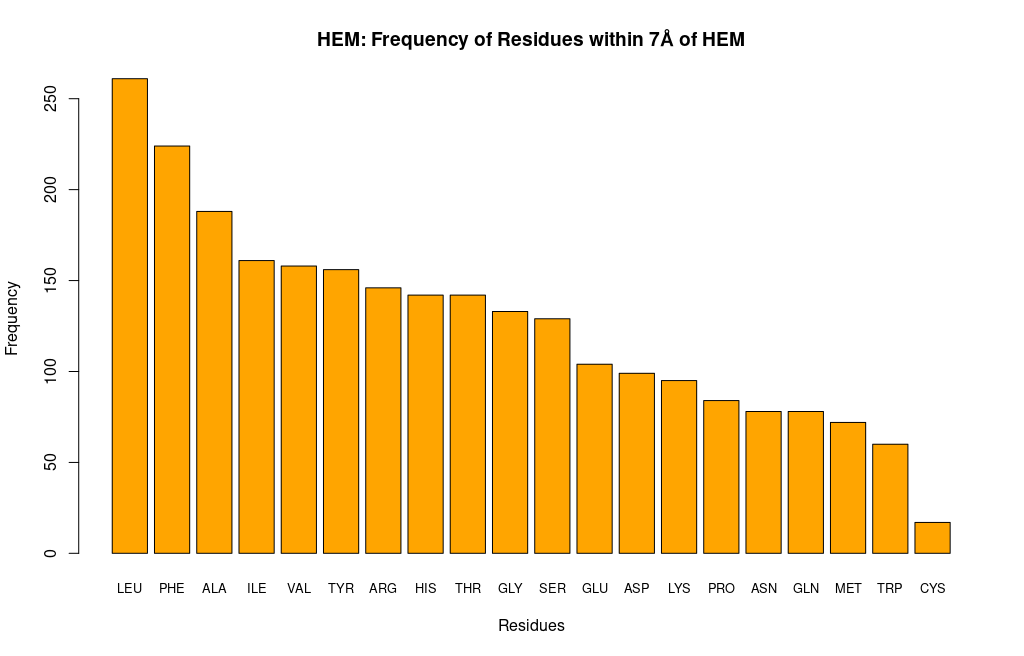
\includegraphics[width=1.0\textwidth]{7A/HEM_aaFreq}
		%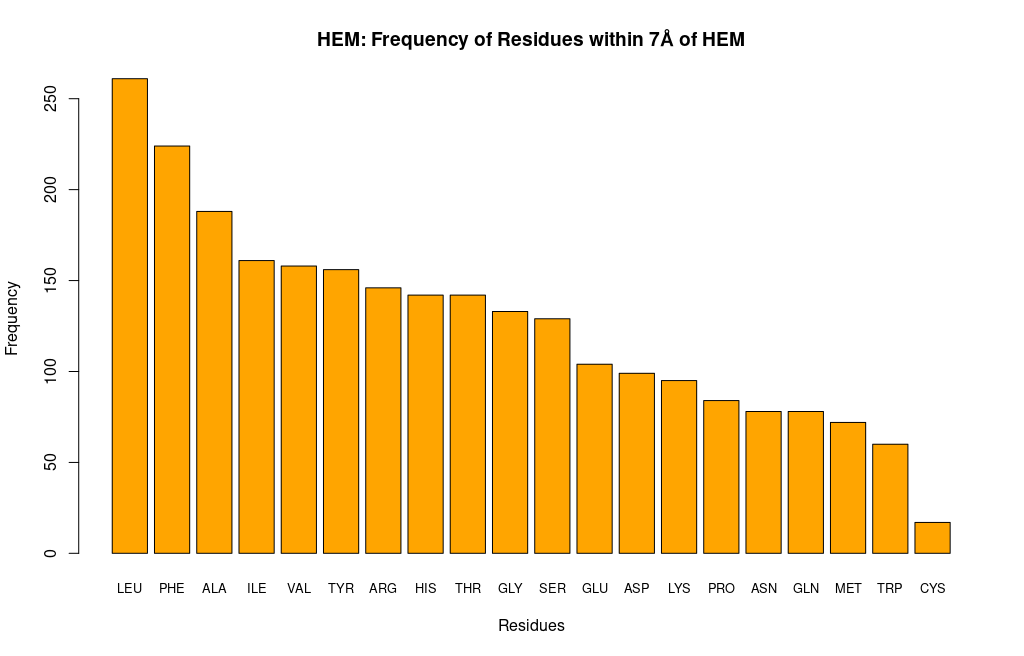
\includegraphics{~/heme-binding/thesis/figures/fuckinghell}
	\end{figure}
	
	\begin{figure}
		\caption{HEC AA Frequency 7A}
		\label{figs:HEC_aafreq7}
		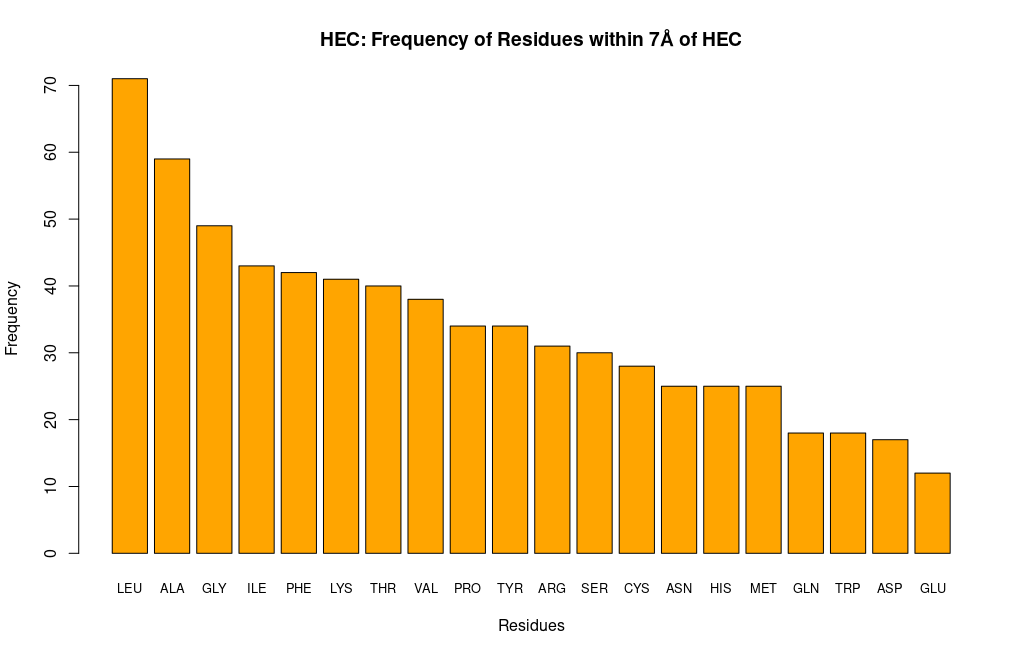
\includegraphics[width=1.0\textwidth]{7A/HEC_aaFreq}
	\end{figure}
		
	\begin{figure}
		\caption{SRM AA Frequency 7A}
		\label{figs:SRM_aafreq7}
		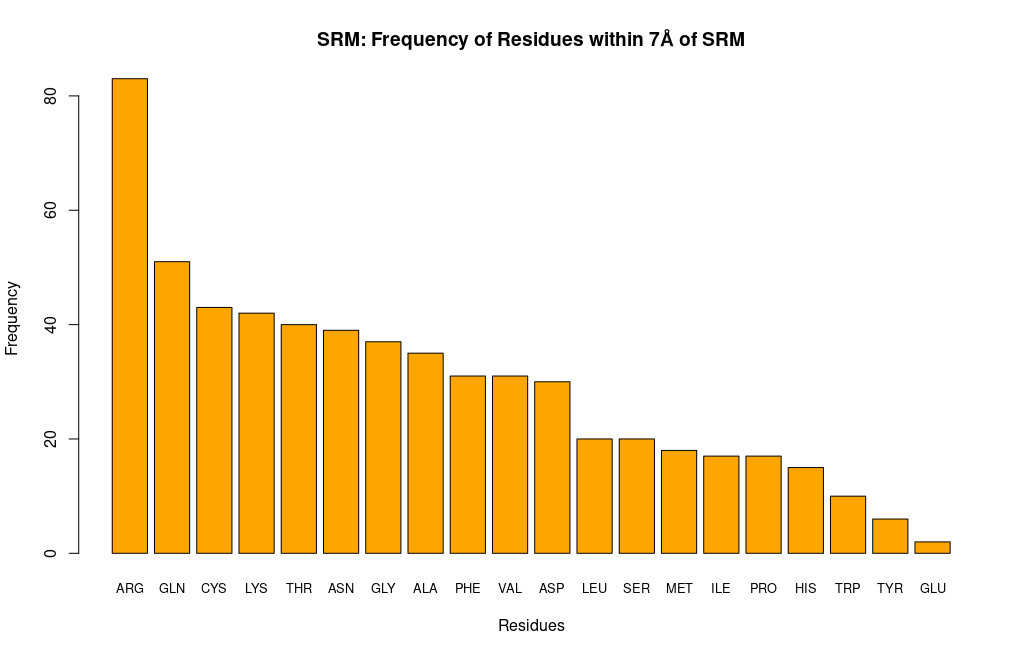
\includegraphics[width=1.0\textwidth]{7A/SRM_aaFreq}
	\end{figure}
	
	\begin{figure}
		\caption{VERDOHEME AA Frequency 7A}
		\label{figs:VERDOHEME_aafreq7}
		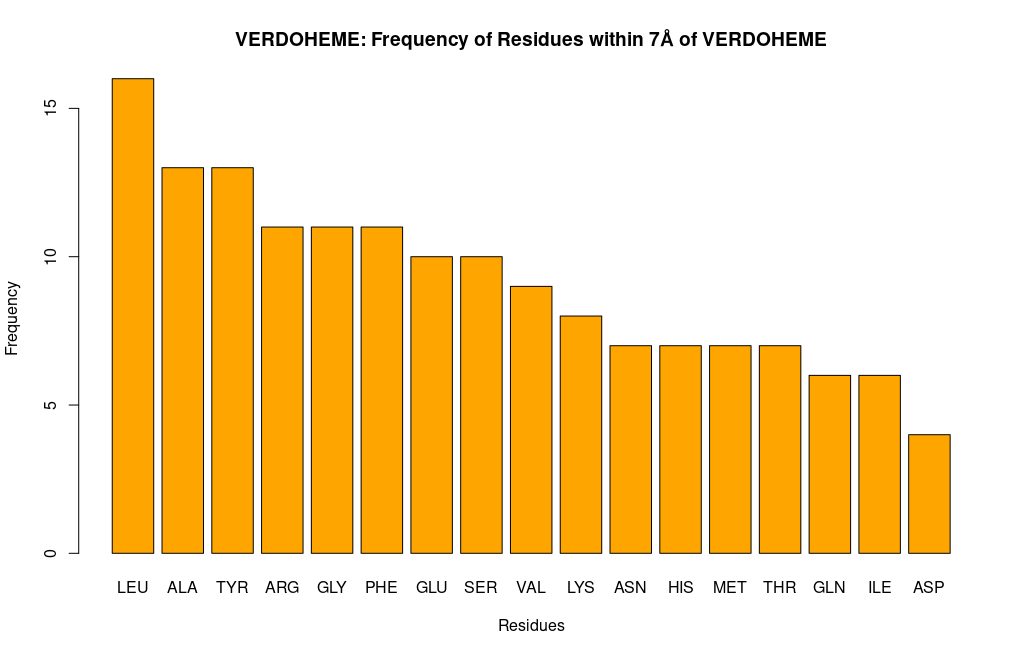
\includegraphics[width=1.0\textwidth]{7A/VERDOHEME_aaFreq}
	\end{figure}



		
\section{CACBFe Data}
	\begin{figure}
		\caption{HEM CACBFe Data}
		\label{figs:HEM_cab7}
		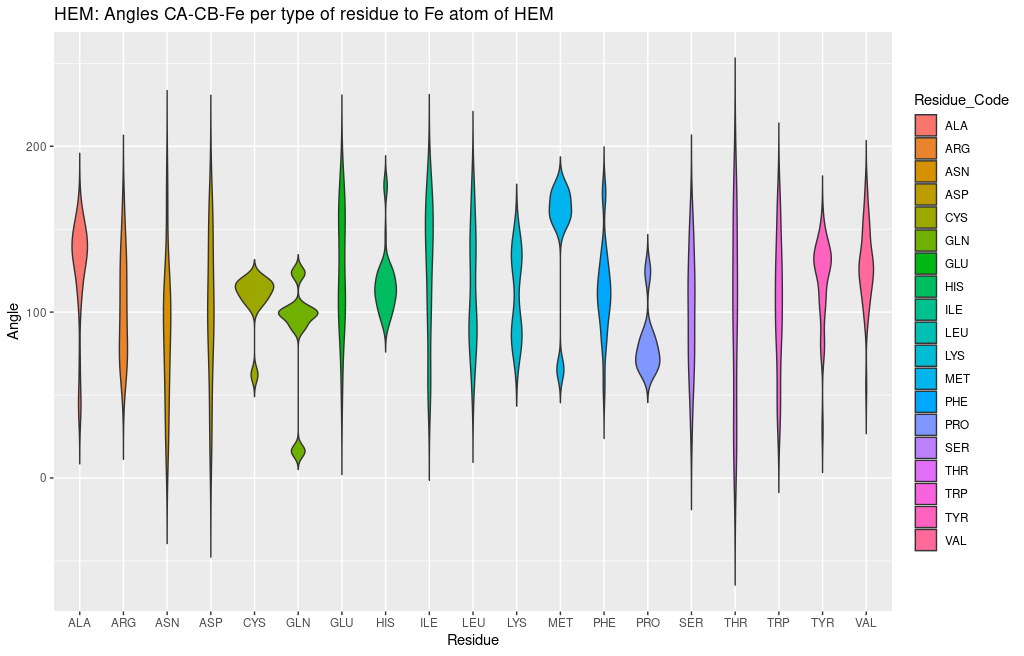
\includegraphics[width=\linewidth]{7A/HEM_cab}
	\end{figure}

	\begin{figure}
		\caption{HEC CACBFe Data}
		\label{figs:HEC_cab7}
		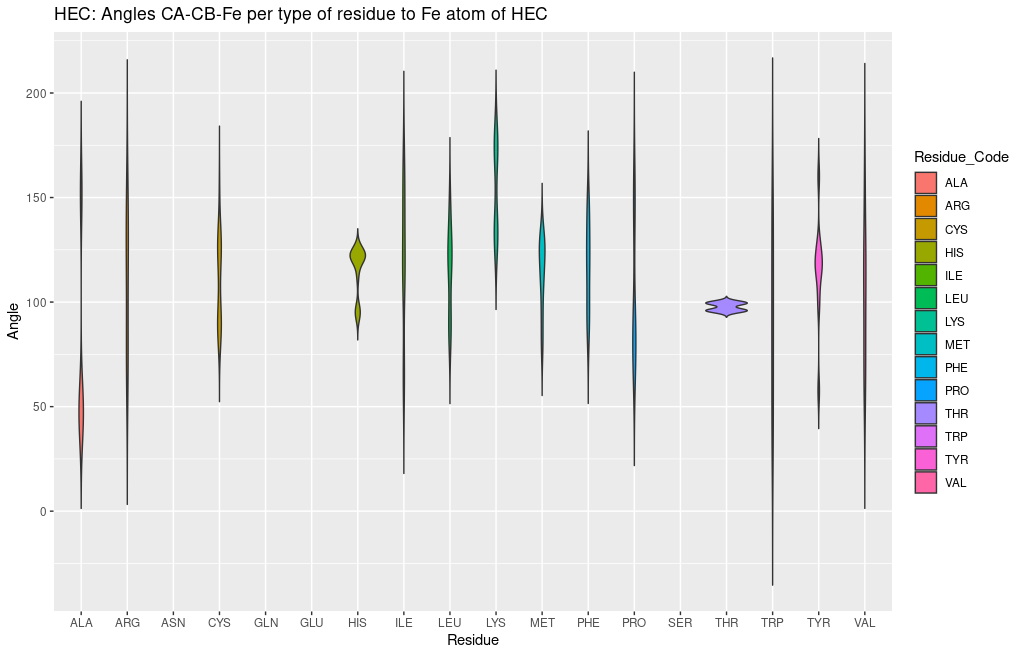
\includegraphics[width=\linewidth]{7A/HEC_cab}
	\end{figure}
	
	\begin{figure}
		\caption{SRM CACBFe Data}
		\label{figs:SRM_cab7}
		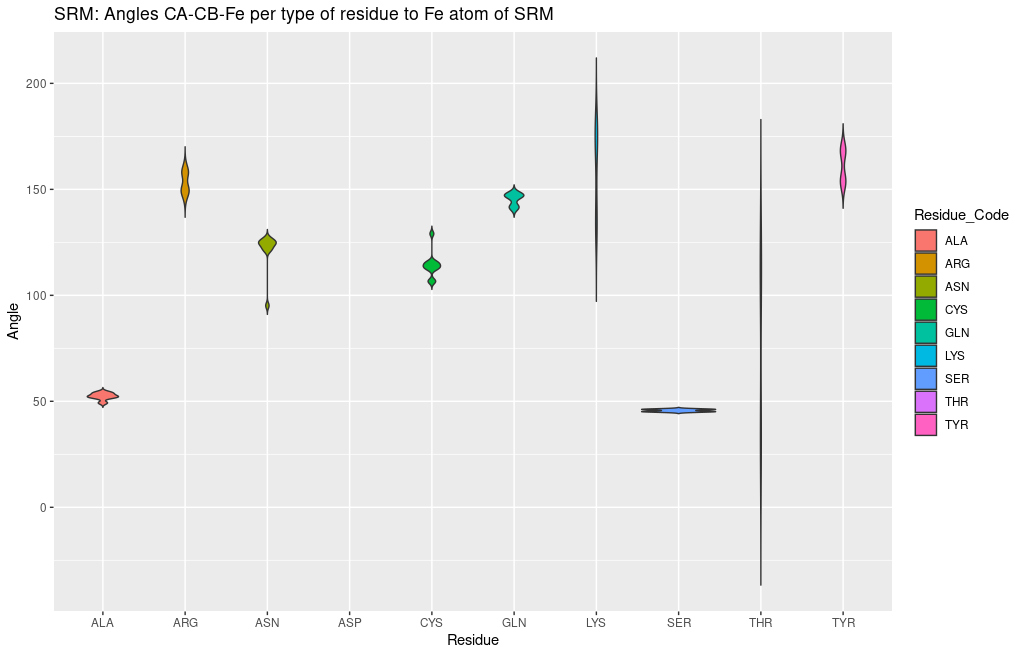
\includegraphics[width=\linewidth]{7A/SRM_cab}
	\end{figure}
	
	\begin{figure}
		\caption{VERDOHEME CACBFe Data}
		\label{figs:VERDOHEME_cab7}
		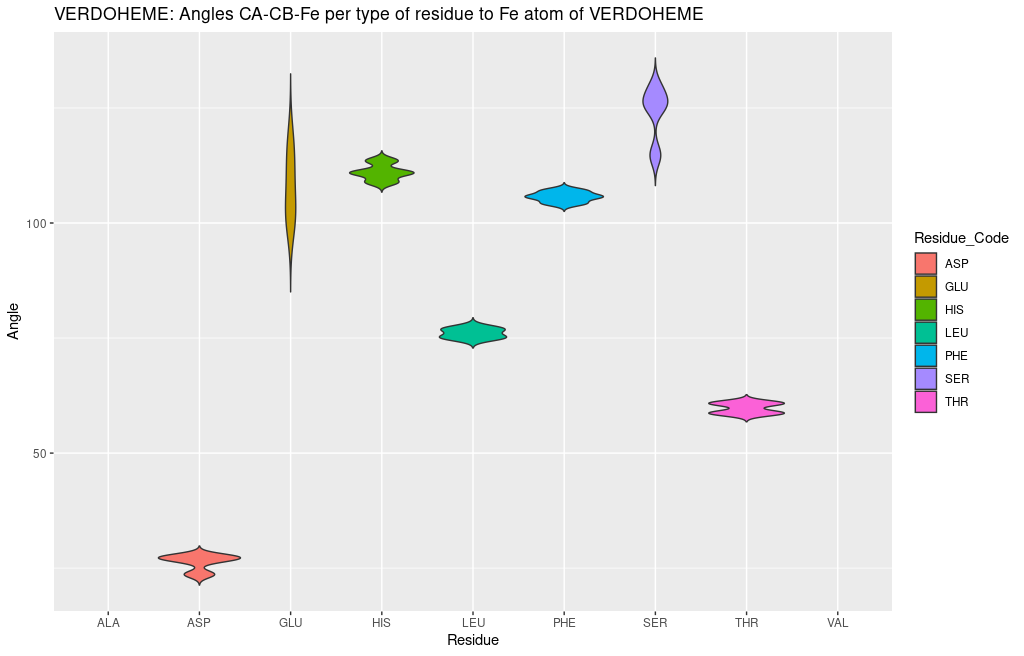
\includegraphics[width=\linewidth]{7A/VERDOHEME_cab}
	\end{figure}
	
\section{Closest Residue Data}
	\begin{figure}
		\caption{HEM Closest Residue Data}
		\label{figs:HEM_closestRes7}
		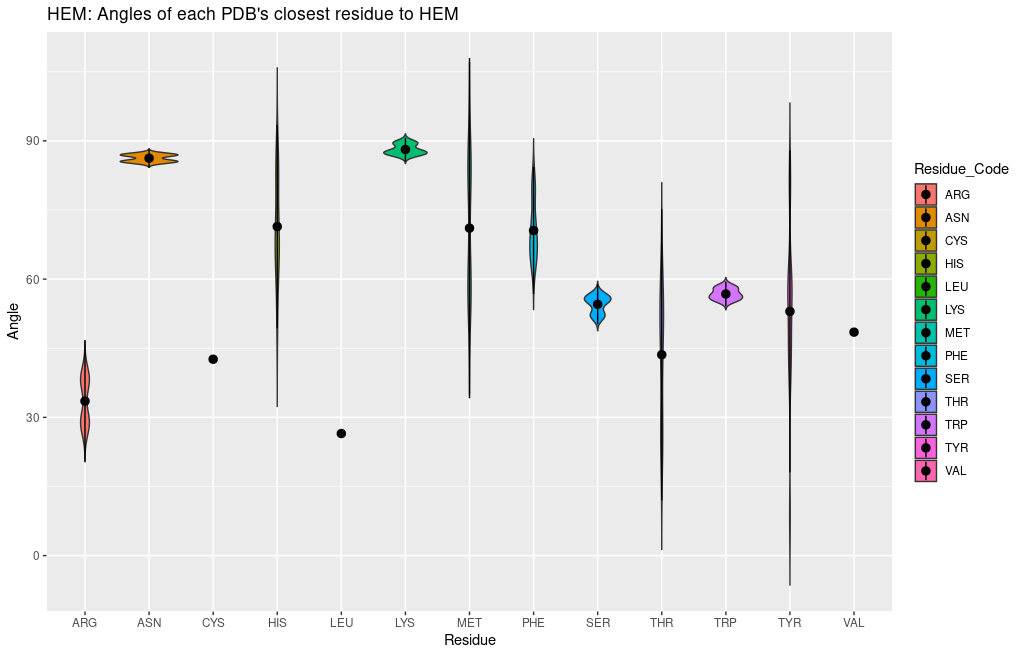
\includegraphics[width=\linewidth]{7A/HEM_closestRes}
	\end{figure}
	
	\begin{figure}
		\caption{HEC Closest Residue Data}
		\label{figs:HEC_closestRes7}
		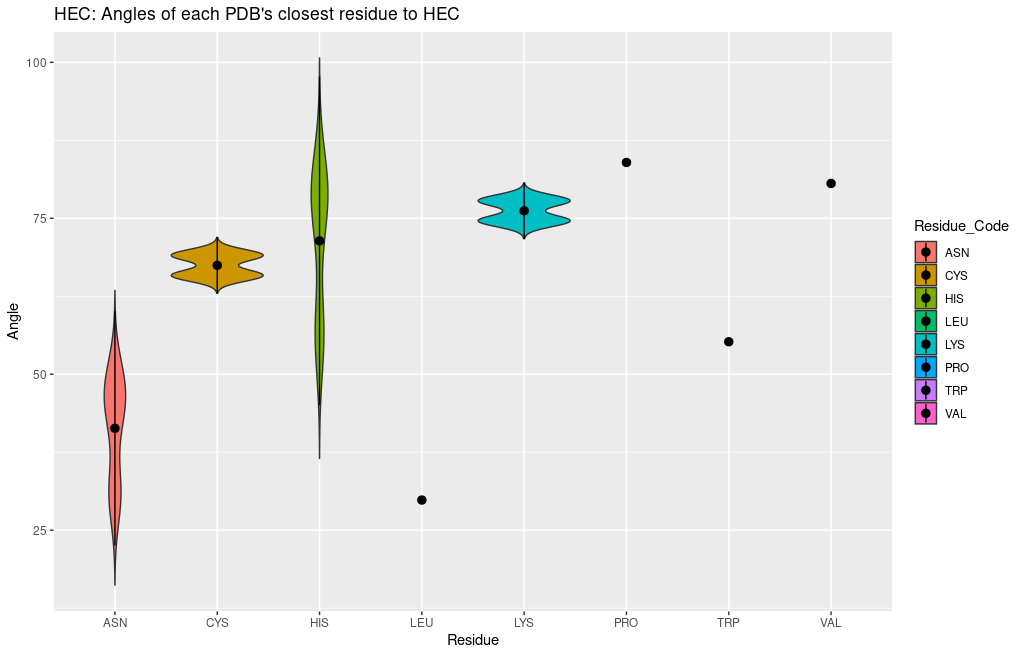
\includegraphics[width=\linewidth]{7A/HEC_closestRes}
	\end{figure}
	
	
	\begin{figure}
		\caption{SRM Closest Residue Data}
		\label{figs:SRM_closestRes7}
		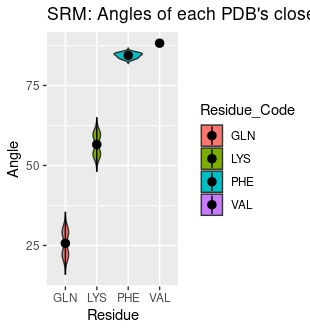
\includegraphics[width=\linewidth]{7A/SRM_closestRes}
	\end{figure}


	\begin{figure}
		\caption{VERDOHEME Closest Residue Data}
		\label{figs:VERDOHEME_closestRes7}
		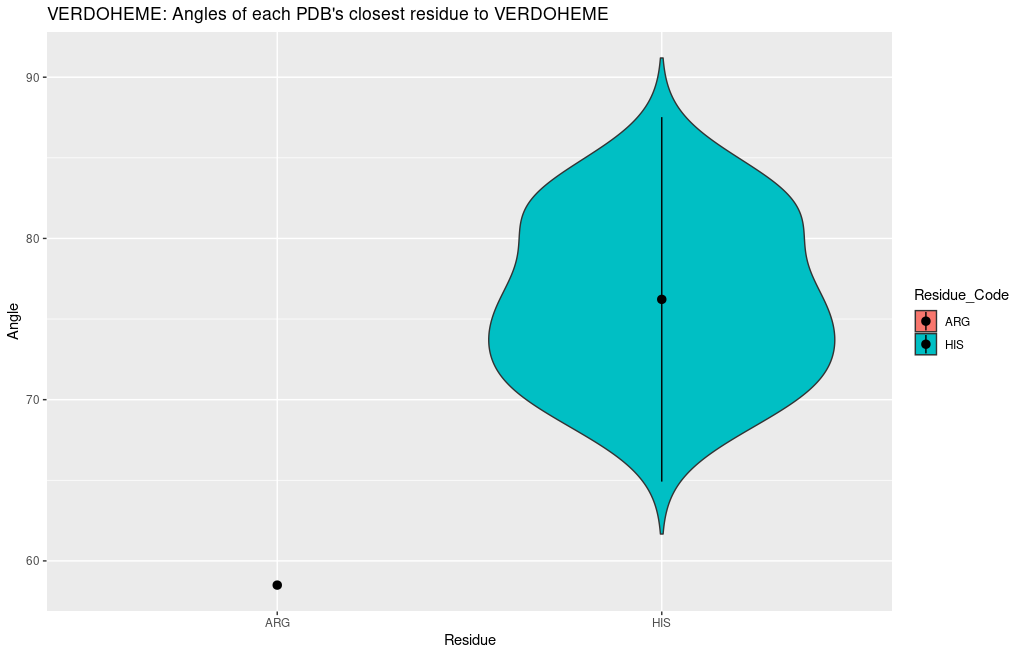
\includegraphics[width=\linewidth]{7A/VERDOHEME_closestRes}
	\end{figure}


\section{Coordinating Residue Data}
	\begin{figure}
		\caption{HEM Coordinating Residue Data}
		\label{figs:HEM_coordRes7}
		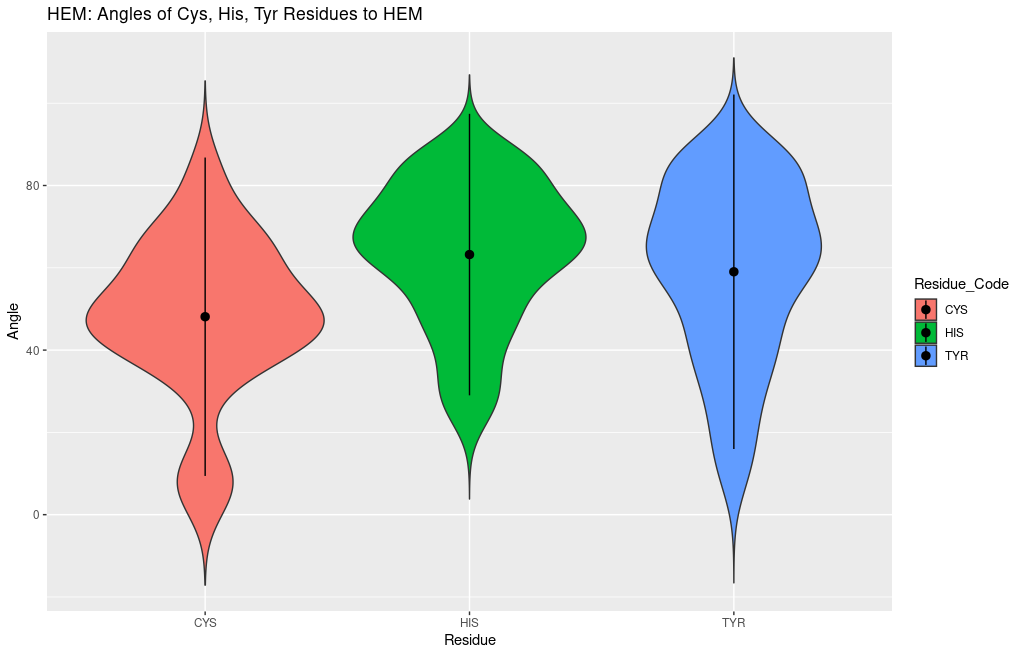
\includegraphics[width=\linewidth]{7A/HEM_coordRes}
	\end{figure}
	
	\begin{figure}
		\caption{HEC Coordinating Residue Data}
		\label{figs:HEC_coordRes7}
		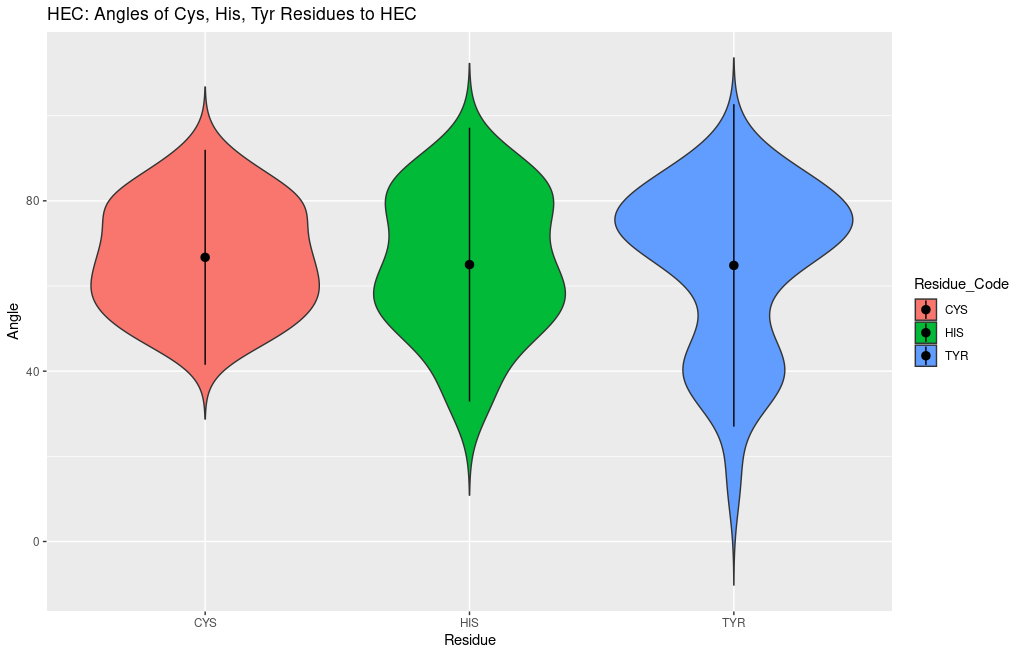
\includegraphics[width=\linewidth]{7A/HEC_coordRes}
	\end{figure}	
		
	\begin{figure}
		\caption{SRM Coordinating Residue Data}
		\label{figs:SRM_coordRes7}
		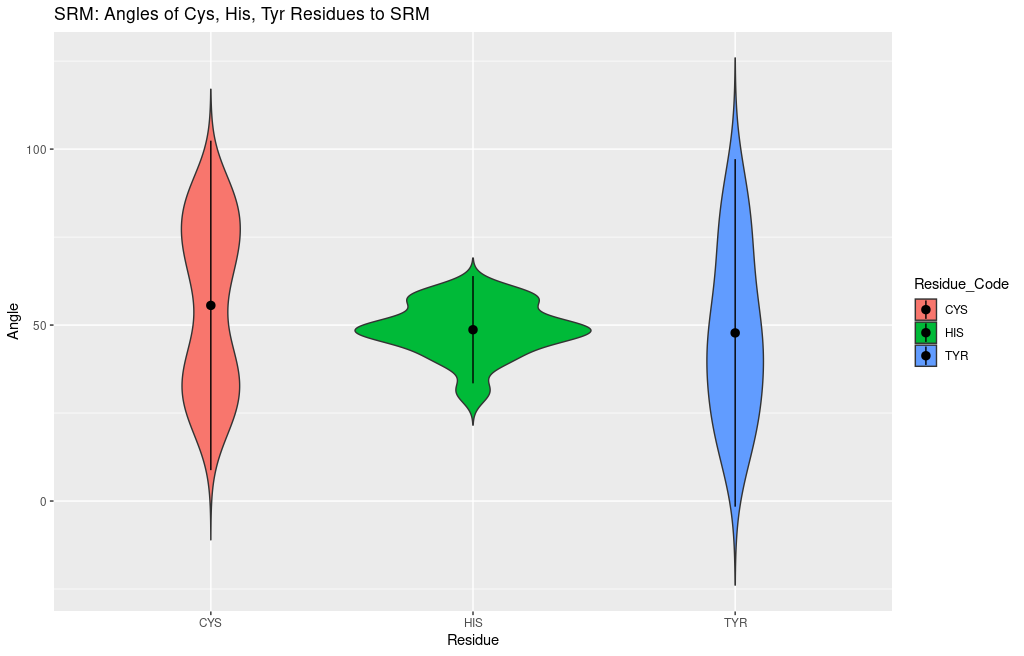
\includegraphics[width=\linewidth]{7A/SRM_coordRes}
	\end{figure}
		
	\begin{figure}
		\caption{VERDOHEME Coordinating Residue Data}
		\label{figs:VERDOHEME_coordRes7}
		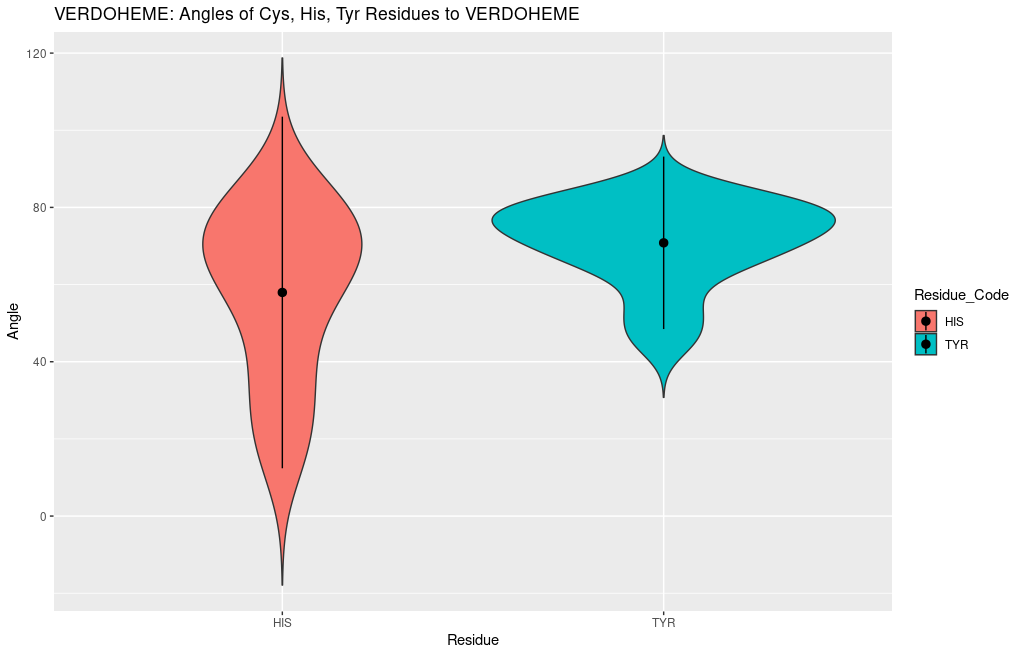
\includegraphics[width=\linewidth]{7A/VERDOHEME_coordRes}
	\end{figure}


\section{Ligand Accessible Surface Area}
	\begin{figure}
		\caption{HEM Ligand Accessible Surface Area}
		\label{figs:HEM_ligandAccSA}
			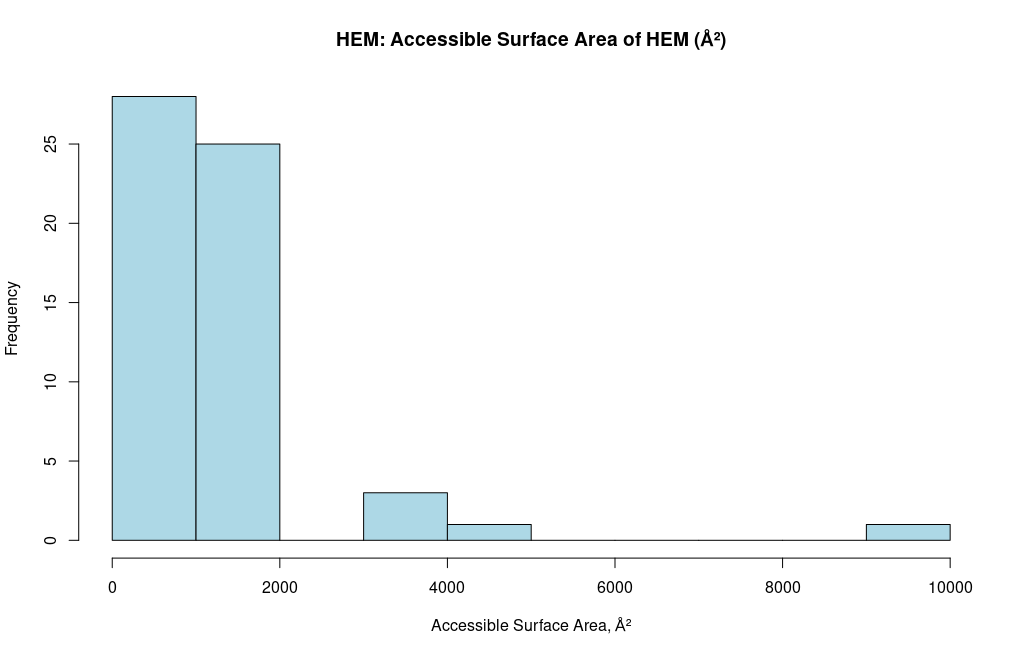
\includegraphics[width=\linewidth]{7A/HEM_ligandAccSA}
	\end{figure}

	\begin{figure}
		\caption{HEC Ligand Accessible Surface Area}
		\label{figs:HEC_ligandAccSA}
		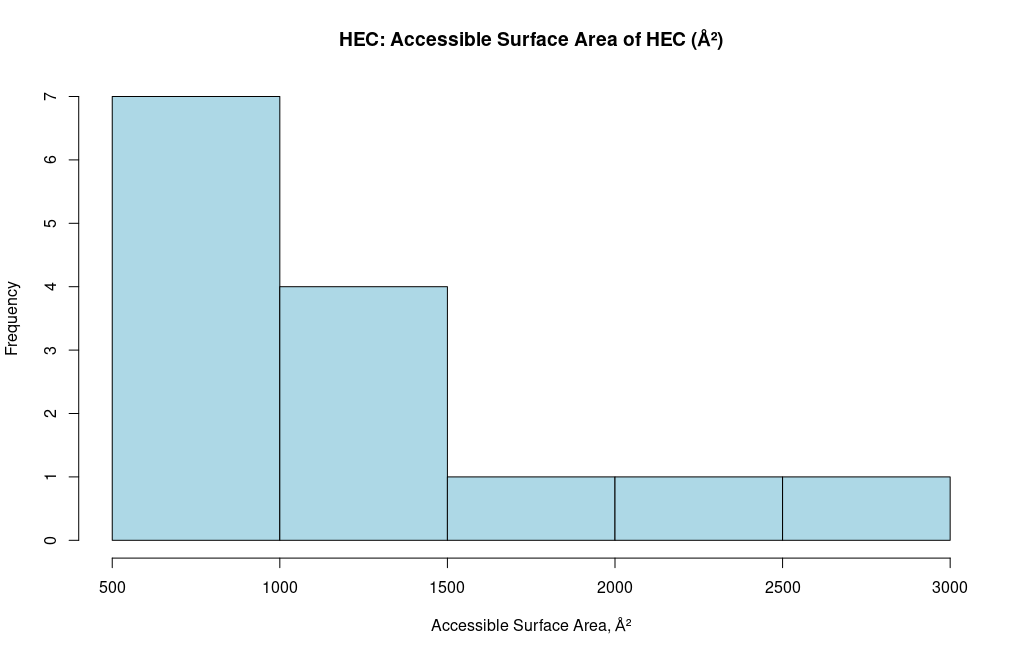
\includegraphics[width=\linewidth]{7A/HEC_ligandAccSA}
	\end{figure}

	\begin{figure}
		\caption{SRM Ligand Accessible Surface Area}
		\label{figs:SRM_ligandAccSA}
		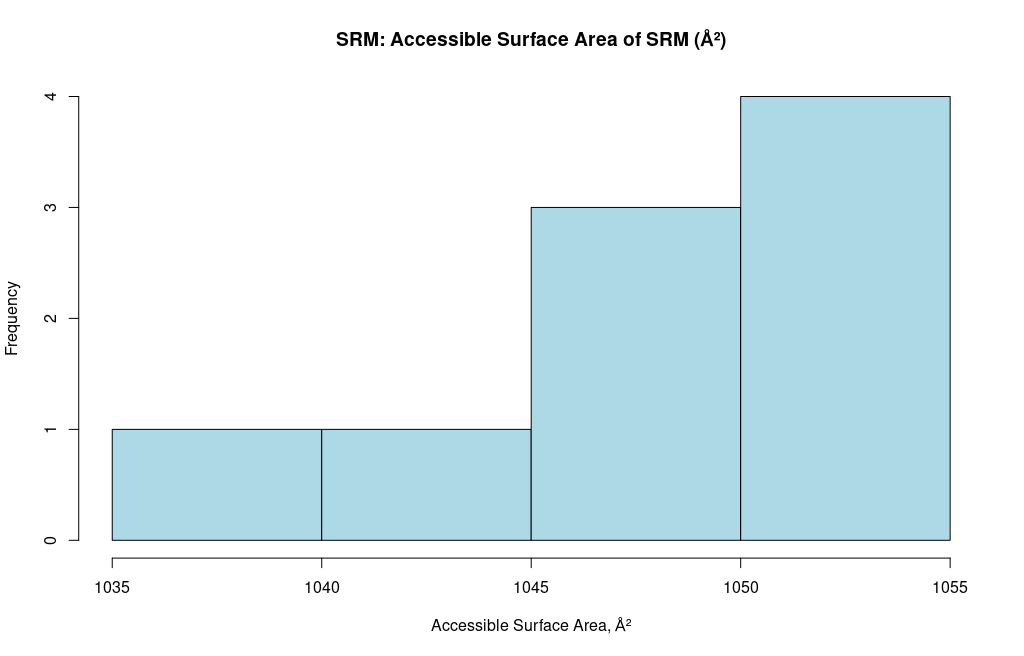
\includegraphics[width=\linewidth]{7A/SRM_ligandAccSA}
	\end{figure}

	\begin{figure}
		\caption{VERDOHEME Ligand Accessible Surface Area}
		\label{figs:VERDOHEME_ligandAccSA}
		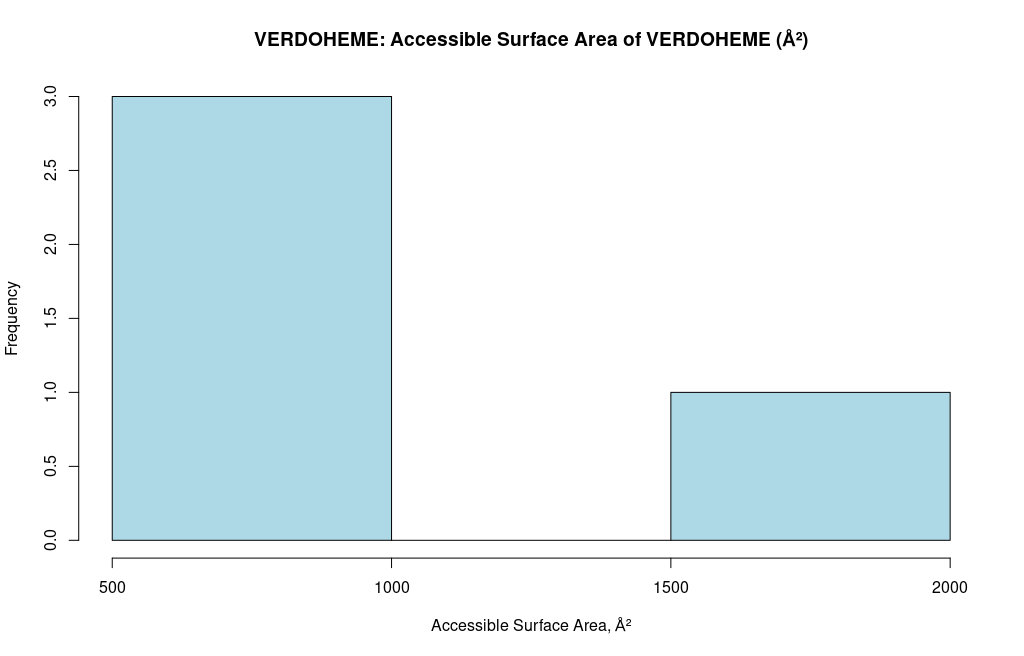
\includegraphics[width=\linewidth]{7A/VERDOHEME_ligandAccSA}
	\end{figure}

\section{Ligand Excluded Surface Area}
	\begin{figure}
		\caption{HEM Ligand Excluded Surface Area}
		\label{figs:HEM_ligandExcSA}
		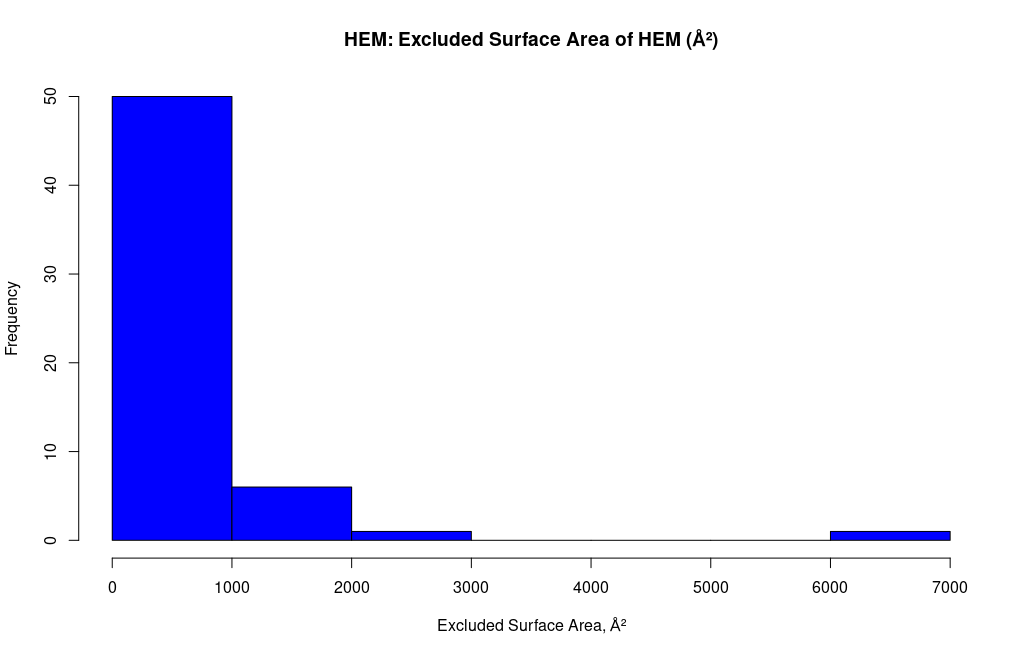
\includegraphics[width=\linewidth]{7A/HEM_ligandExcSA}
	\end{figure}
	
	\begin{figure}
		\caption{HEC Ligand Excluded Surface Area}
		\label{figs:HEC_ligandExcSA}
		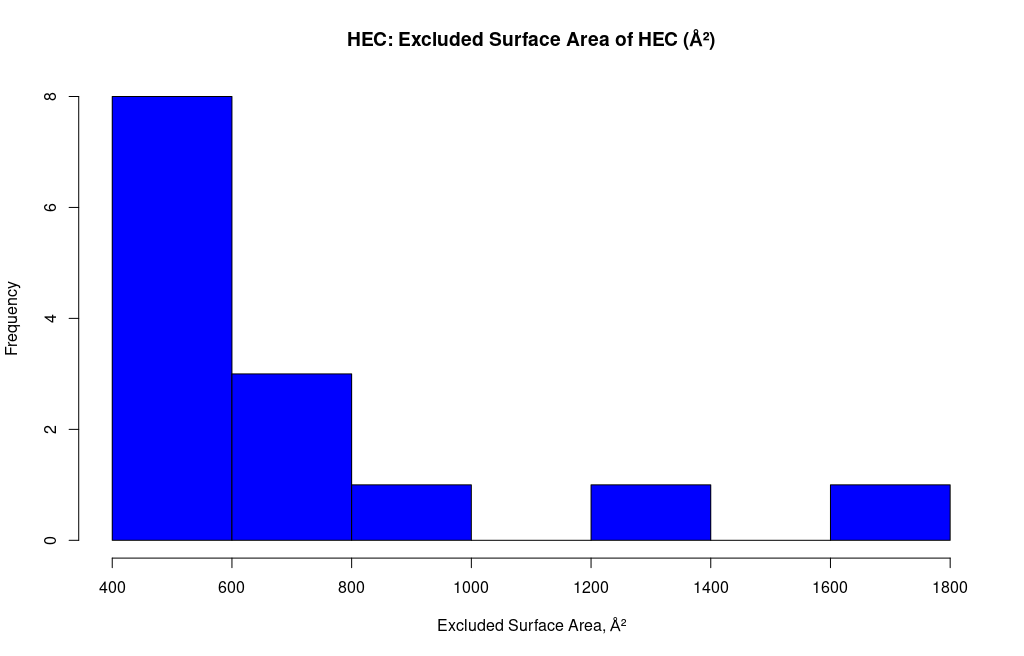
\includegraphics[width=\linewidth]{7A/HEC_ligandExcSA}
	\end{figure}

	\begin{figure}
		\caption{SRM Ligand Excluded Surface Area}
		\label{figs:SRM_ligandExcSA}
		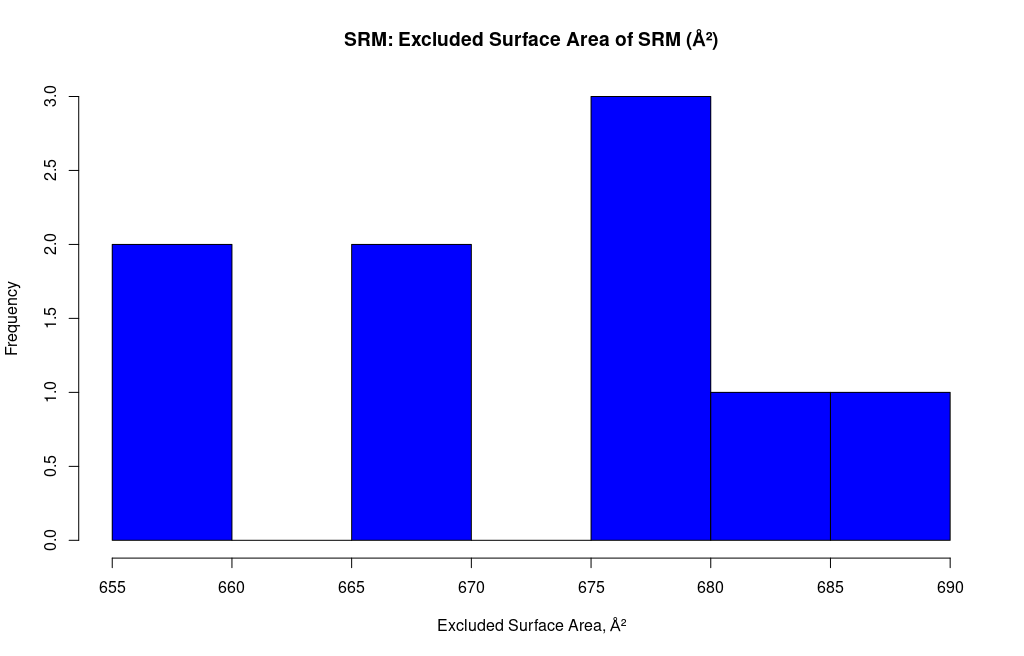
\includegraphics[width=\linewidth]{7A/SRM_ligandExcSA}
	\end{figure}

	\begin{figure}
		\caption{VERDOHEME Ligand Excluded Surface Area}
		\label{figs:VERDOHEME_ligandExcSA}
		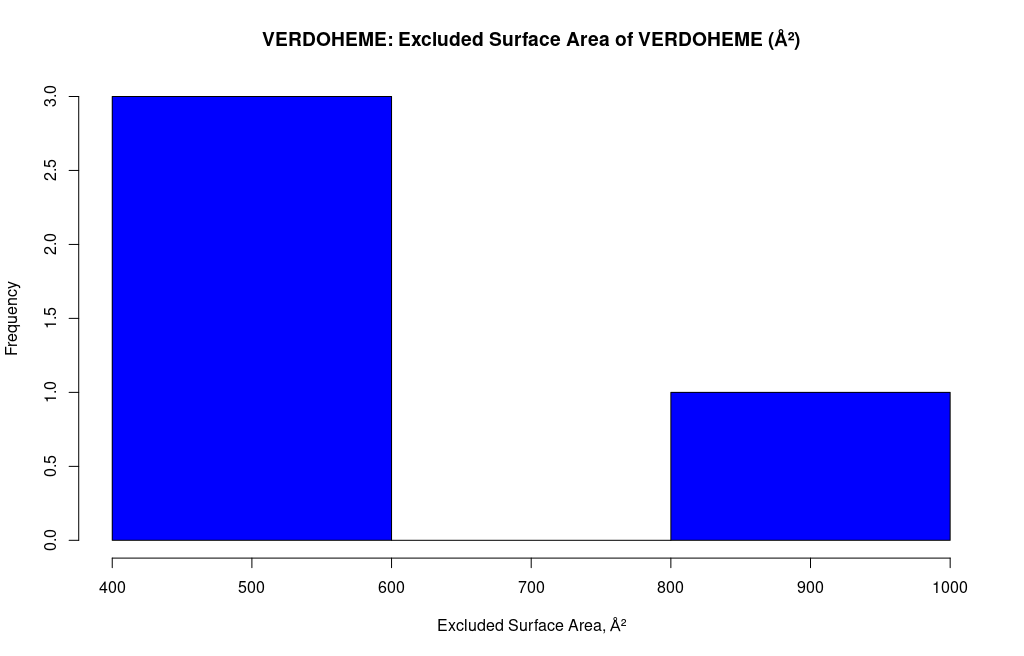
\includegraphics[width=\linewidth]{7A/VERDOHEME_ligandExcSA}
	\end{figure}

\section{Planar Angles}
	\begin{figure}
		\caption{HEM Planar Angles}
		\label{figs:HEM_planarAngles}
		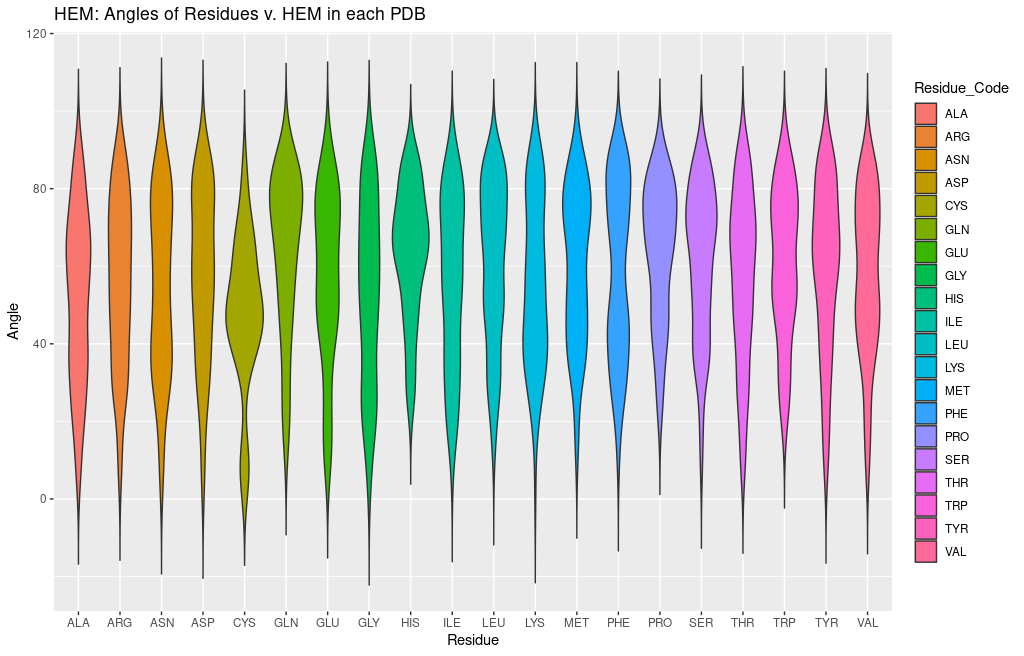
\includegraphics[width=\linewidth]{7A/HEM_planarAngles}
	\end{figure}
	
	\begin{figure}
		\caption{HEC Planar Angles}
		\label{figs:HEC_planarAngles}
		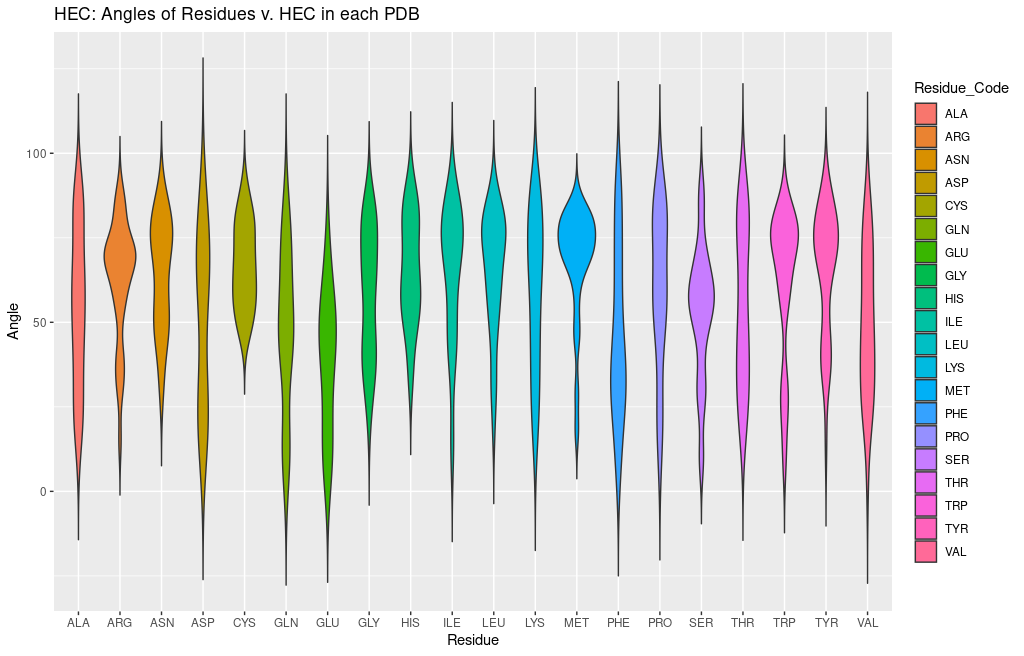
\includegraphics[width=\linewidth]{7A/HEC_planarAngles}
	\end{figure}
	
	\begin{figure}
		\caption{SRM Planar Angles}
		\label{figs:SRM_planarAngles}
		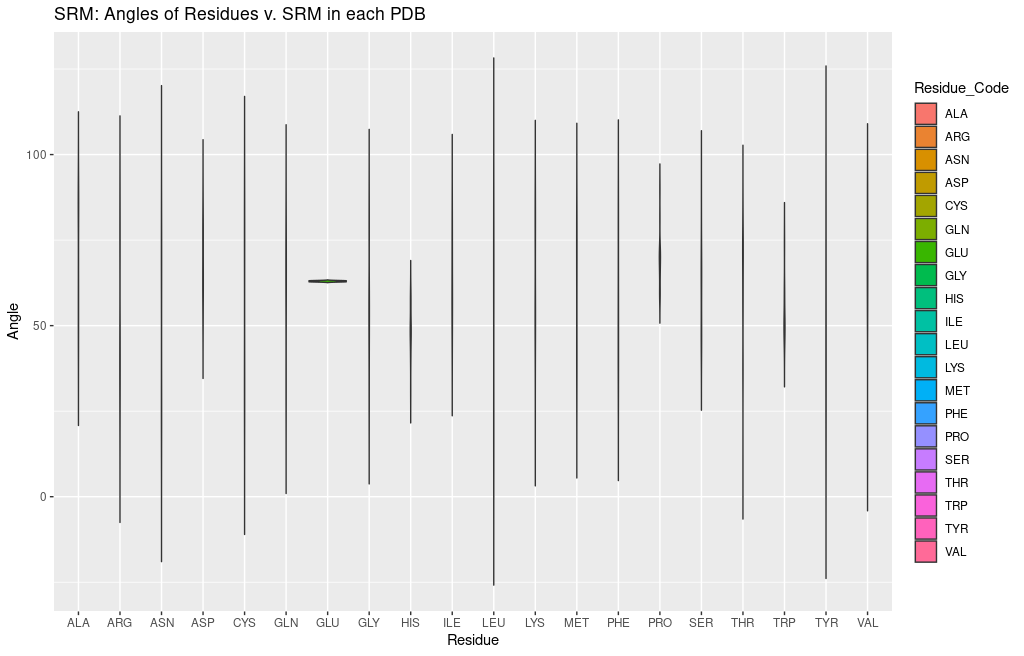
\includegraphics[width=\linewidth]{7A/SRM_planarAngles}
	\end{figure}
	
	\begin{figure}
		\caption{VERDOHEME Planar Angles}
		\label{figs:VERDOHEME_planarAngles}
		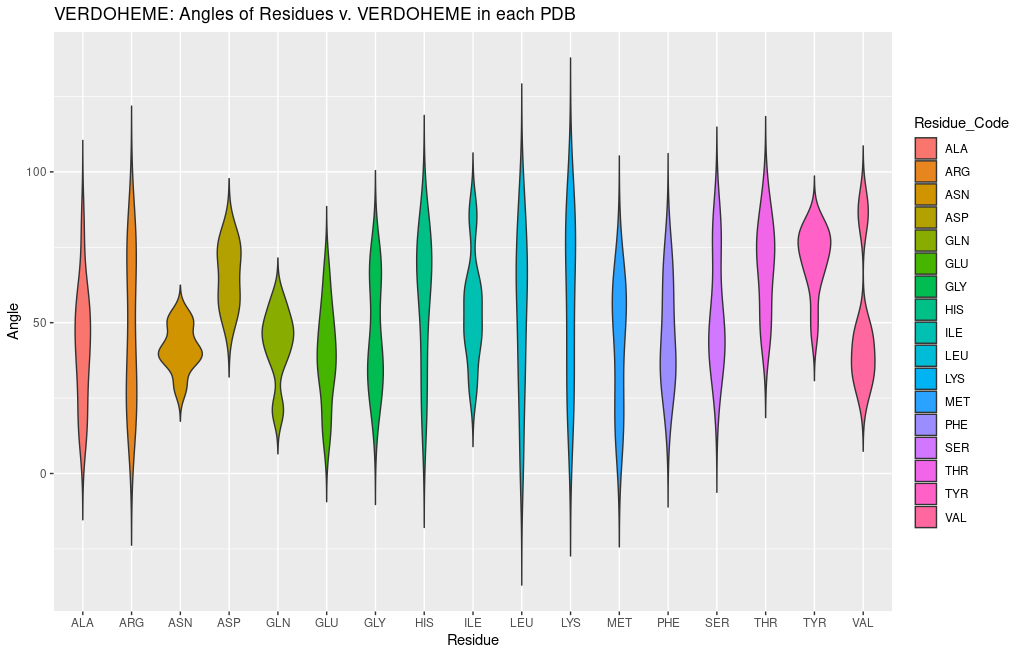
\includegraphics[width=\linewidth]{7A/VERDOHEME_planarAngles}
	\end{figure}
	
\section{Pocket Accessible Surface Area}
	\begin{figure}
		\caption{HEM Pocket Accessible Surface Area}
		\label{figs:HEM_pocketAccSA}
		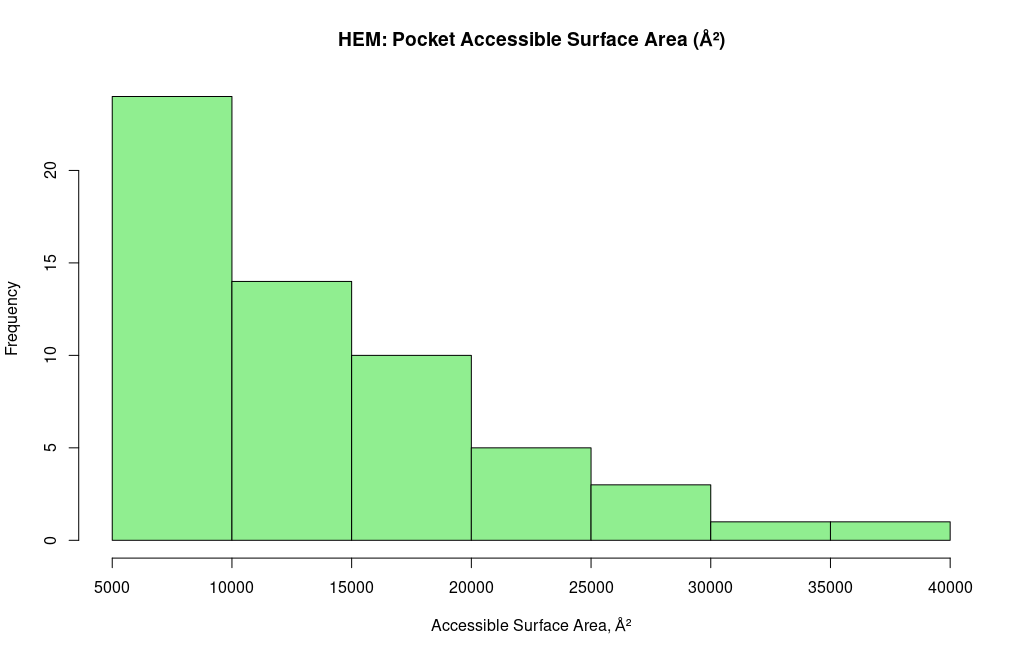
\includegraphics[width=\linewidth]{7A/HEM_pocketAccSA}
	\end{figure}
	% attempt below to have like a four-way square of stuff going on, but it gets pretty tiny... and probs not necessary

% belows prevent latex from adding whitespace automatically

%\begin{figure}%
%	\centering
%	\subfloat[\centering num1]{{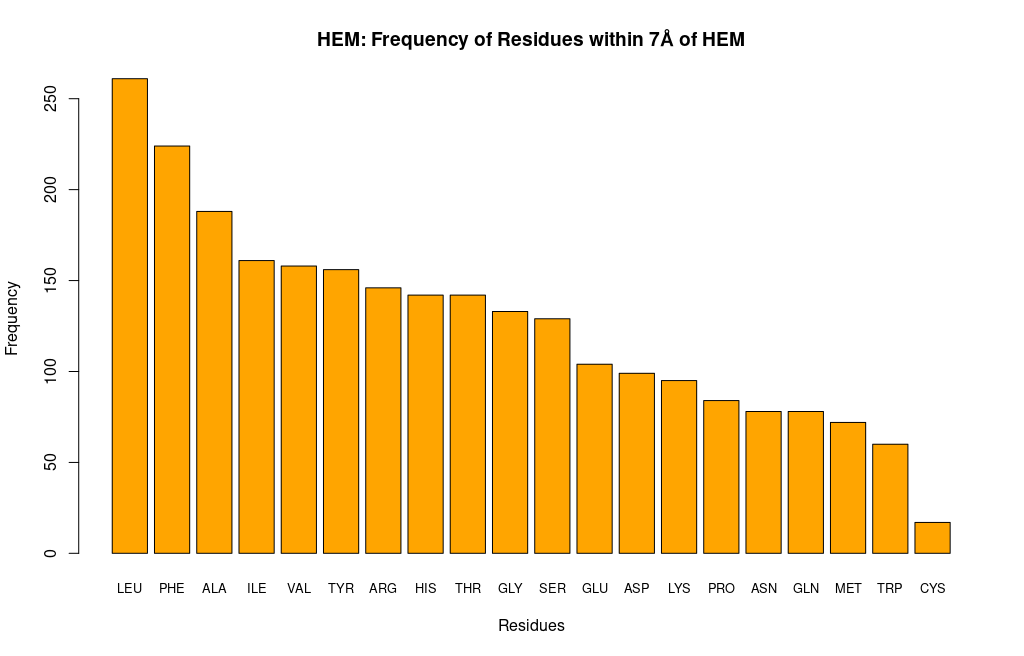
\includegraphics[width=5cm]{7A/HEM_aaFreq}}}%
%	\qquad
%	\subfloat[\centering num2]{{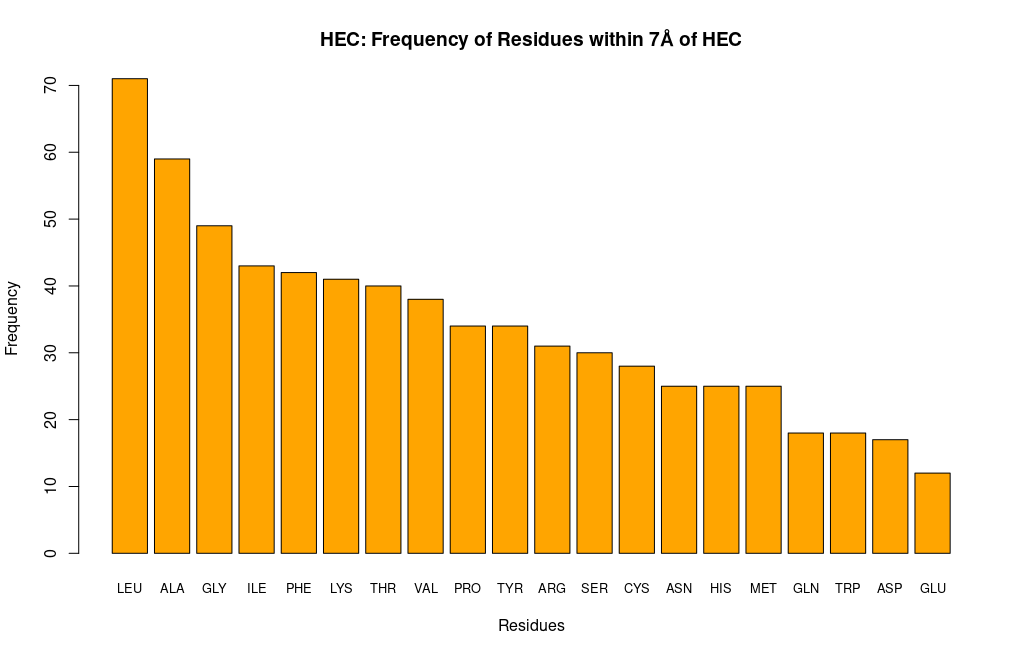
\includegraphics[width=1.0\textwidth]{7A/HEC_aaFreq}}}%
%	\caption{These are two shits}%
%	label{fig:allAAFreq}%
%\end{figure}